We now return to the case study outlined in section \ref{sec:casestudy}. Our surveillance task is $\LTLsquare \LTLdiamond p_5$, i.e, we need to infinitely often bring the belief of the target location to 5 cells or lower. We partition the gridworld in figure \ref{fig:SGR-grid} as shown in figure \ref{fig:experiment}.

\begin{figure}
\centering
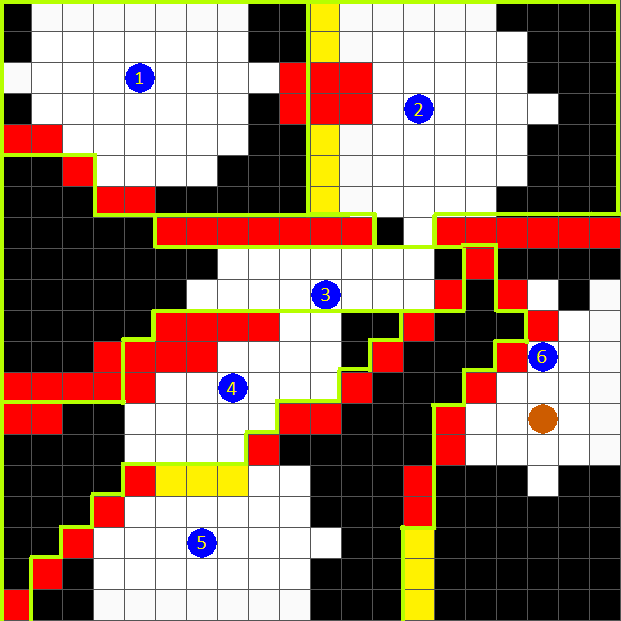
\includegraphics[scale=0.2]{figs/SGR-grid-vis-part.png}
\caption{The gridworld in \ref{fig:SGR-grid}}
\label{fig:experiment}
\end{figure}

Using this partition, we have 6 subgames. 